\documentclass[11pt,a4paper]{article}

\usepackage[margin=1in]{geometry}
\usepackage{amsmath,amssymb}
\usepackage{booktabs}
\usepackage{caption}
\usepackage{enumitem}
\usepackage{float}
\usepackage{graphicx}
\usepackage{hyperref}
\usepackage{longtable}
\usepackage{subcaption}
\usepackage{xcolor}

\hypersetup{
    colorlinks=true,
    linkcolor=blue,
    citecolor=blue,
    urlcolor=blue
}

\setlist[itemize]{leftmargin=1.4em}
\setlist[enumerate]{leftmargin=1.6em}
\graphicspath{{figures/}}

\title{\textbf{Quantitative Trading Strategy Report}\\
\large LGBM, GRPO and GARCH-Bollinger Strategies on HSI Futures}
\author{STAT8020 Quantitative Strategies and Algorithmic Trading}
\date{\today}

\begin{document}

\maketitle
\tableofcontents
\newpage

\section{Introduction}

This project studies whether intraday Hang Seng Index (HSI) futures prices contain exploitable short-term patterns after transaction costs and execution frictions. The theoretical starting point is the Efficient Market Hypothesis (EMH). Under weak-form and semi-strong-form efficiency, prices should already reflect historical prices and public information, so persistent abnormal returns should be difficult to obtain. In practice, intraday markets can still display temporary predictability because of liquidity imbalance, volatility clustering, investor overreaction, market microstructure noise, and delayed information diffusion across day and night sessions.

The project compares three trading approaches. The first is a supervised learning strategy based on LightGBM (LGBM), which predicts next-bar returns from engineered price, volatility, volume, and calendar features. The second is a reinforcement learning strategy based on a GRPO-style policy optimization framework, where a policy network learns whether to be short, flat, or long from trading rewards. The third is a traditional GARCH-Bollinger strategy, which combines Bollinger Bands with GARCH conditional volatility, volume confirmation, and session-specific parameter selection.

The report follows the style of the sample project reports: it starts from market theory and trading rationale, then defines strategy rules, describes in-sample and out-of-sample design, presents parameter optimization, and finally discusses backtesting results, slippage, risk management, and implementation difficulties.

\begin{figure}[H]
    \centering
    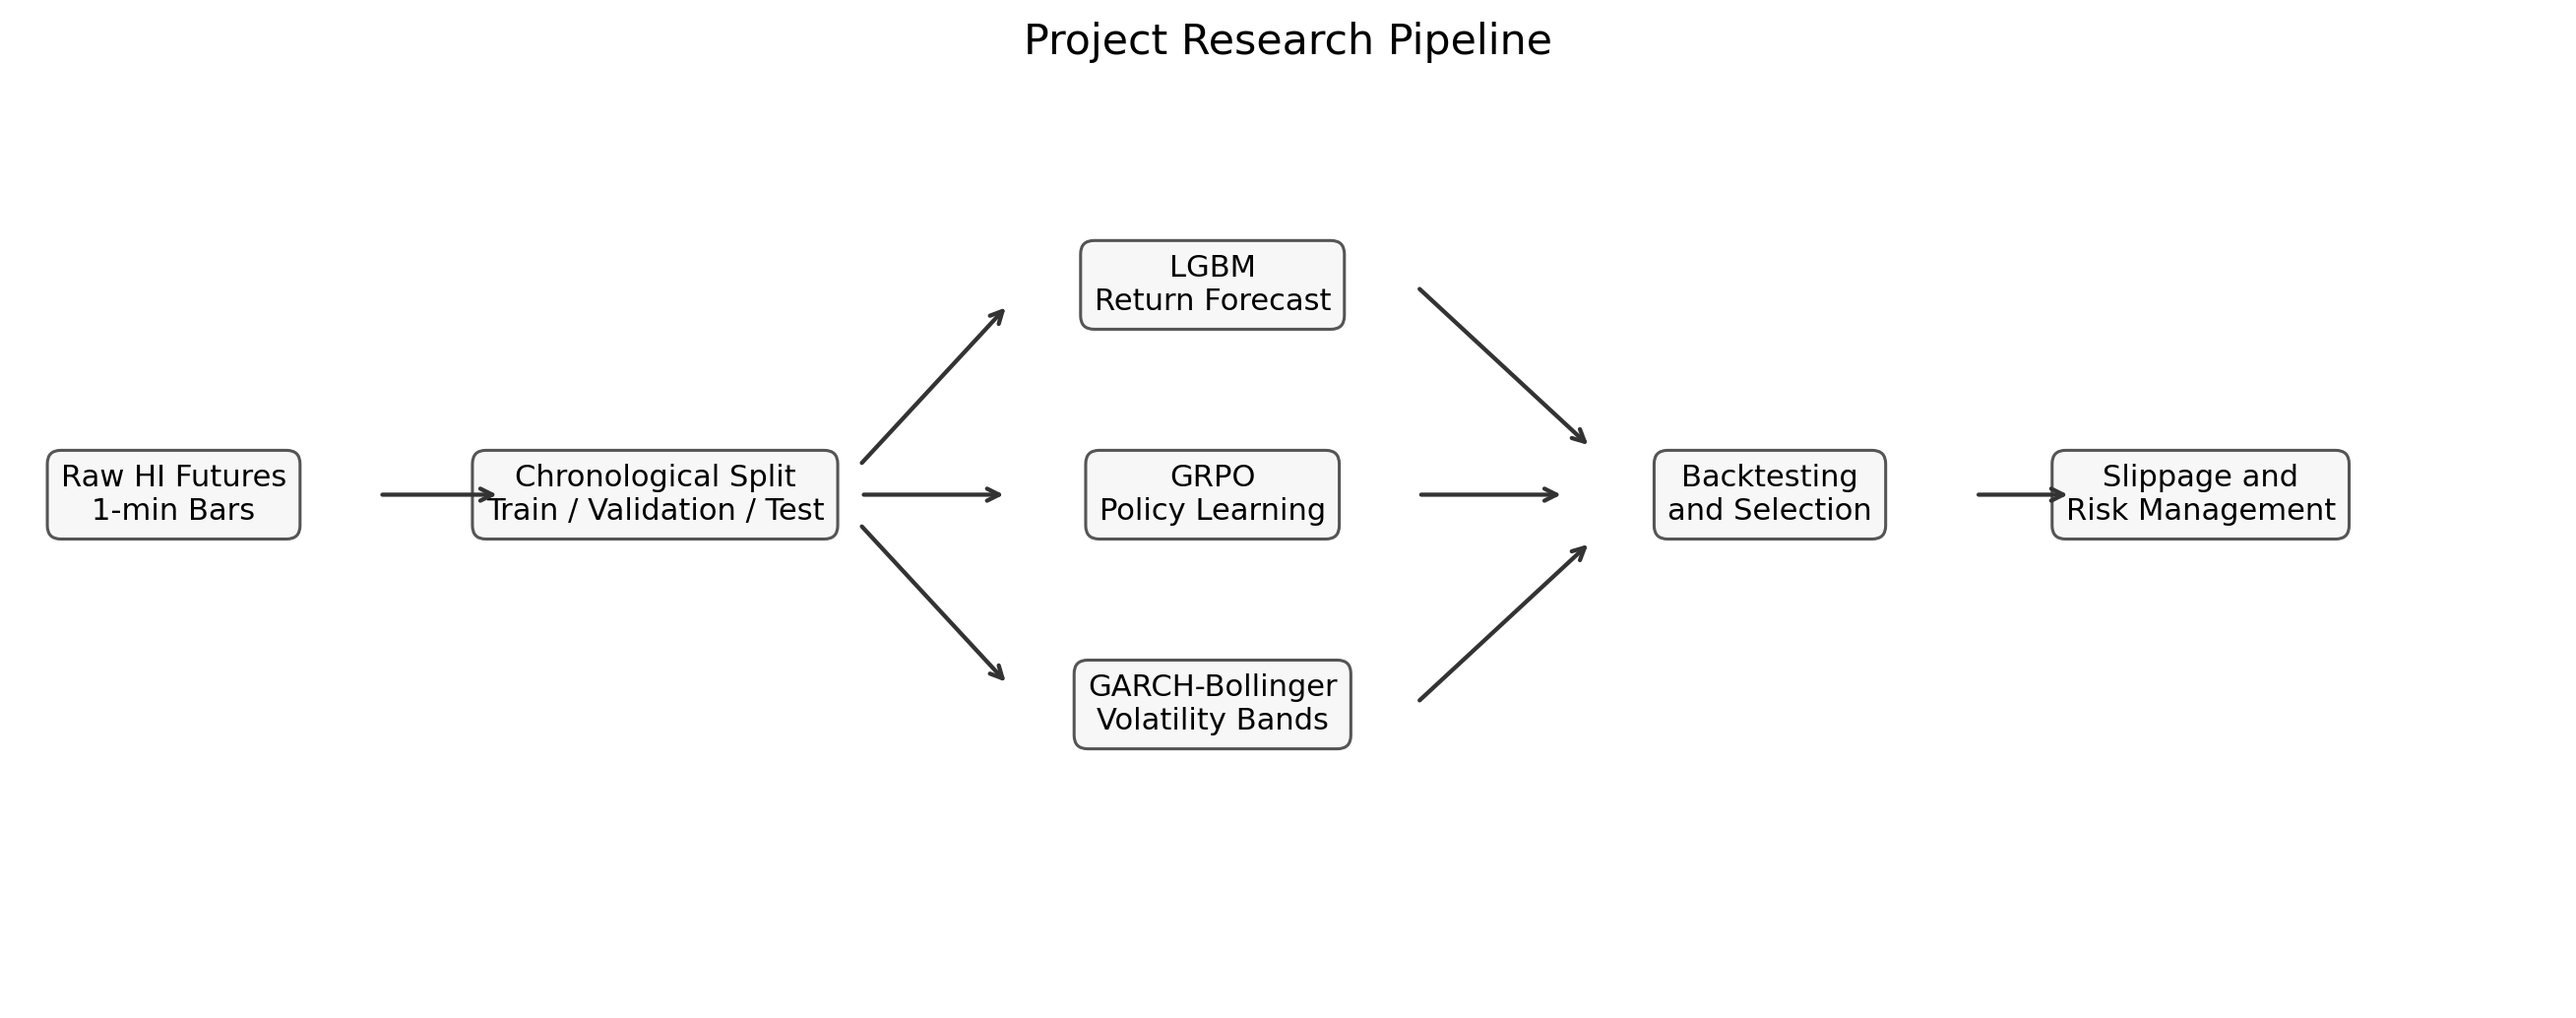
\includegraphics[width=0.95\textwidth]{project_workflow.png}
    \caption{Research pipeline from processed HSI futures data to model training, backtesting, risk management and final comparison.}
    \label{fig:workflow}
\end{figure}

\section{Trading Algorithms and Rationale}

\subsection{LGBM Supervised Learning Strategy}

The LGBM strategy treats trading as a short-horizon return prediction problem. The prediction target is the next-minute close-to-close return:

\begin{equation}
    y_t = \frac{P_{t+1}}{P_t} - 1.
\end{equation}

The model is a LightGBM gradient boosting regressor. It is suitable for this task because tree boosting can model nonlinear interactions among technical indicators, volume variables, volatility measures, and time-of-day effects without requiring a linear return model.

The feature set contains 41 variables. They include lagged returns, log returns, rolling volatility, volume moving averages and volume ratios, candlestick shape variables, moving averages, moving-average deviations, moving-average crosses, RSI-style variables, and intraday calendar encodings. The feature design follows several economic intuitions:

\begin{itemize}
    \item Lagged returns and moving-average deviations capture momentum and reversal.
    \item Rolling volatility captures volatility clustering.
    \item Volume ratios capture liquidity and market participation.
    \item Hour, minute-of-day and day-of-week encodings capture intraday seasonality.
\end{itemize}

The trading rule converts predicted returns into positions only when the expected return is large enough to cover round-trip cost:

\begin{equation}
    q_t =
    \begin{cases}
        +1, & \hat{y}_t > c_t,\\
        -1, & \hat{y}_t < -c_t,\\
        0, & \text{otherwise},
    \end{cases}
\end{equation}

where $q_t$ is the target position and $c_t$ is the transaction-cost and slippage threshold. This cost-aware threshold is important because a small positive return forecast may not be tradable after execution frictions.

\subsection{GRPO Reinforcement Learning Strategy}

The GRPO strategy formulates intraday trading as a sequential decision problem. The trading environment has three discrete actions:

\begin{equation}
    a_t \in \{0,1,2\}, \qquad 0=\text{short}, \quad 1=\text{flat}, \quad 2=\text{long}.
\end{equation}

The environment maps these actions to target positions $\{-1,0,+1\}$. At each step, the environment calculates futures PnL using the current and next bar prices:

\begin{align}
    \mathrm{GrossPnL}_t &= q_t(P_{t+1}-P_t)M,\\
    \mathrm{Cost}_t &= |q_t-q_{t-1}|(C + sM),\\
    \mathrm{NetPnL}_t &= \mathrm{GrossPnL}_t - \mathrm{Cost}_t,\\
    r_t &= \frac{\mathrm{NetPnL}_t}{\mathrm{InitialCapital}},
\end{align}

where $M=50$ is the HSI futures multiplier, $C$ is fixed transaction cost per contract, and $s$ is slippage in index points.

The observation vector contains standardized market features and the current position. Feature means and standard deviations are computed from the training set and saved with the model. The same normalization is then reused during validation, testing, and risk management, which avoids distribution leakage from the test set.

The optimization follows a GRPO-style relative reward idea. For a group of sampled episodes, the advantage of episode $i$ is:

\begin{equation}
    A_i = \frac{R_i - \bar{R}}{\sigma_R + \epsilon},
\end{equation}

where $R_i$ is the total episode return. The policy loss is:

\begin{equation}
    \mathcal{L} = -\frac{1}{N}\sum_i A_i \sum_t \log \pi_\theta(a_{i,t}|s_{i,t}) - \lambda H(\pi_\theta).
\end{equation}

This design rewards policies that outperform other sampled trajectories in the same group. The entropy term encourages exploration and reduces premature convergence.

\subsection{GARCH-Bollinger Strategy}

The GARCH-Bollinger strategy is an interpretable benchmark. A standard Bollinger Band uses a moving average and rolling standard deviation:

\begin{align}
    \mathrm{MA}_t &= \mathrm{RollingMean}(P_t, w)_{t-1},\\
    \mathrm{Upper}_t &= \mathrm{MA}_t + k\sigma^{\mathrm{roll}}_t,\\
    \mathrm{Lower}_t &= \mathrm{MA}_t - k\sigma^{\mathrm{roll}}_t.
\end{align}

The one-period shift is essential: the band used for the decision at time $t$ must be known before observing the trading result at time $t$.

The project extends the band width using GARCH(1,1) conditional volatility:

\begin{align}
    r_t &= \sigma_t z_t,\\
    \sigma_t^2 &= \omega + \alpha r_{t-1}^2 + \beta \sigma_{t-1}^2.
\end{align}

Since $\sigma_t$ is return volatility, it is converted back to price scale:

\begin{equation}
    \mathrm{BandWidth}_t = k P_{t-1}\sigma_t.
\end{equation}

Two signal interpretations are tested. The contrarian version treats a band breach as temporary overreaction and trades against the move. The momentum version treats it as a breakout and trades with the move. Some variants add volume confirmation:

\begin{equation}
    \mathrm{VolumeOK}_t = \mathbb{1}\left(V_t > \rho \cdot \mathrm{RollingMean}(V_t, w_v)_{t-1}\right).
\end{equation}

\section{Data Splitting and Experimental Design}

The raw data are HSI futures one-minute bars from July 2017 to June 2020. The project constructs three datasets: the full original dataset, the day-session dataset, and the night-session dataset. Day session includes 09:15-12:00 and 13:00-16:30. Night session includes 17:15 to the next day 03:00.

All datasets are sorted chronologically and split into train, validation, and test sets with a 3:1:1 ratio. Chronological splitting is necessary because random splitting would allow future regimes to leak into the training process.

\begin{figure}[H]
    \centering
    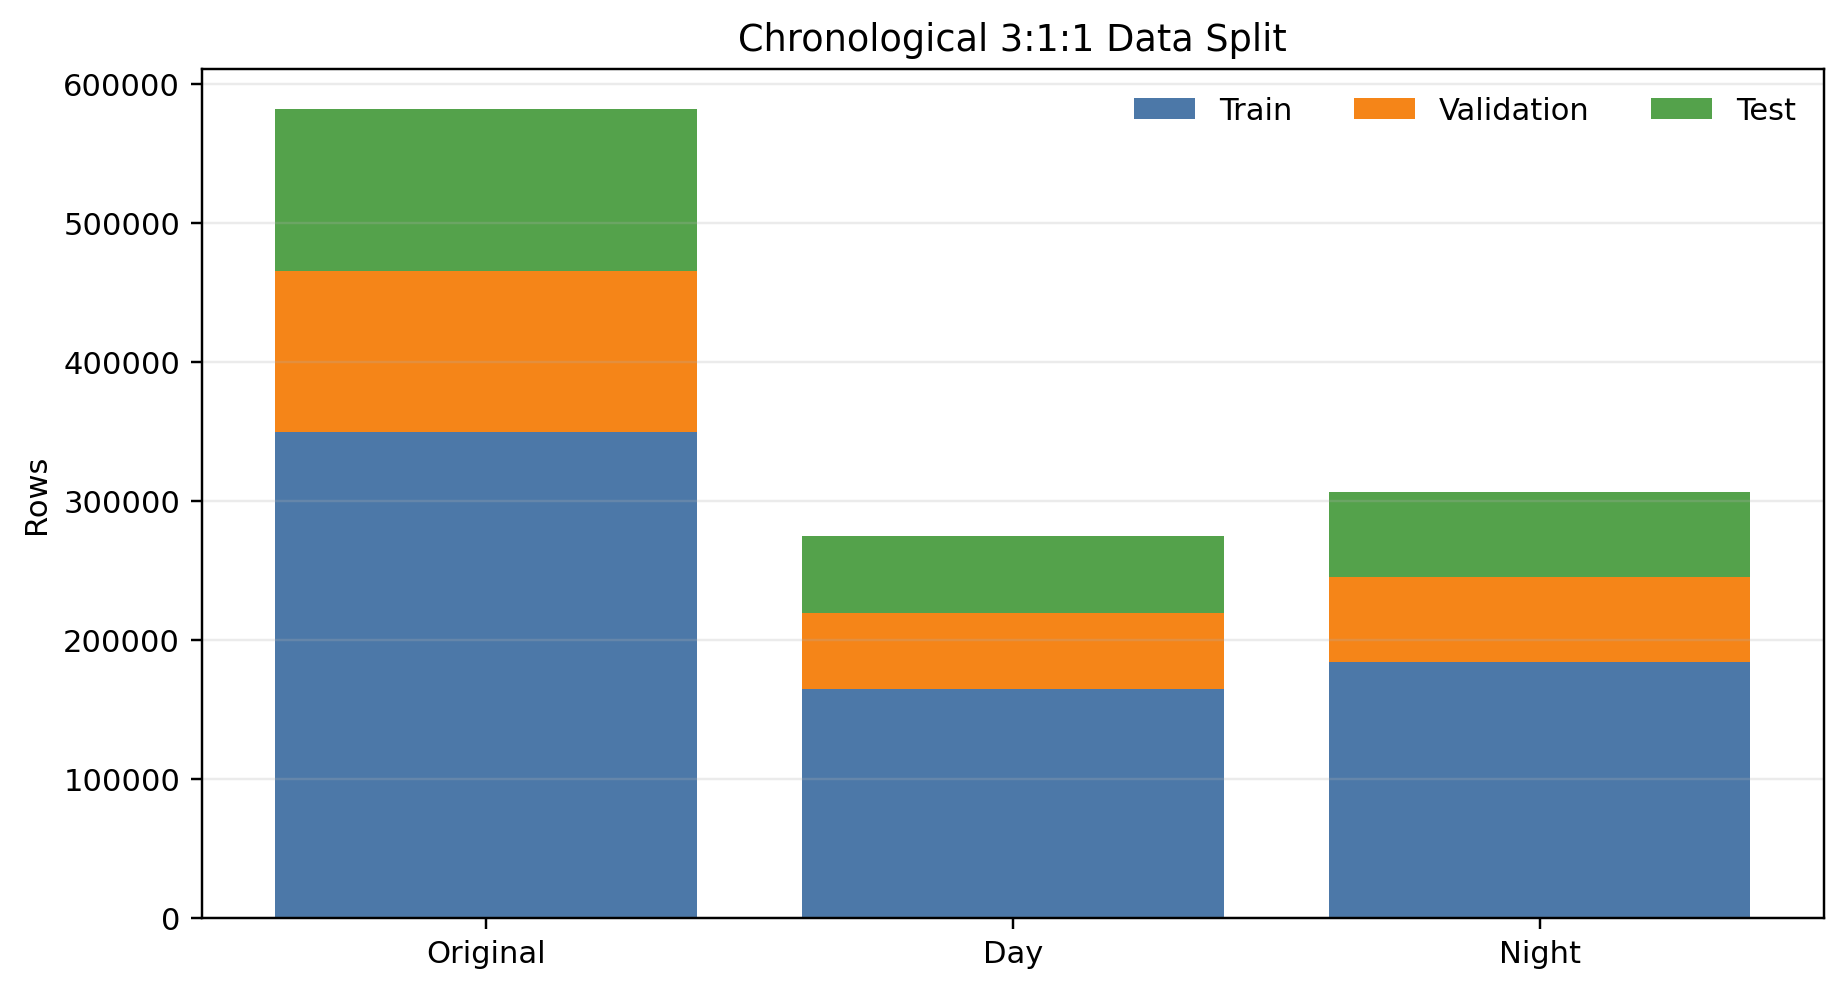
\includegraphics[width=0.82\textwidth]{data_split.png}
    \caption{Chronological train-validation-test split for original, day and night datasets.}
    \label{fig:data-split}
\end{figure}

\begin{table}[H]
    \centering
    \caption{Dataset split summary.}
    \label{tab:split-summary}
    \begin{tabular}{lrrrrll}
        \toprule
        Dataset & Rows & Train & Validation & Test & Start & End \\
        \midrule
        Original & 582100 & 349260 & 116420 & 116420 & 2017-07-03 & 2020-06-09 \\
        Day & 274448 & 164668 & 54890 & 54890 & 2017-07-03 & 2020-06-09 \\
        Night & 306133 & 183679 & 61227 & 61227 & 2017-07-03 & 2020-03-16 \\
        \bottomrule
    \end{tabular}
\end{table}

The roles of the three periods are:

\begin{itemize}
    \item Train: fit model parameters and feature normalization.
    \item Validation: select models, scenarios, and trading parameters.
    \item Test: final out-of-sample evaluation only.
\end{itemize}

\section{Parameter Optimization and Hyperparameter Selection}

\subsection{LGBM Hyperparameter Selection}

The LGBM script uses five-fold \texttt{TimeSeriesSplit}. This preserves time ordering inside cross-validation and is more appropriate than shuffled K-fold validation for financial data. The objective is validation RMSE of next-minute return prediction.

The best parameters selected for all three datasets are:

\begin{table}[H]
    \centering
    \caption{Selected LGBM hyperparameters.}
    \label{tab:lgbm-params}
    \begin{tabular}{lr}
        \toprule
        Hyperparameter & Value \\
        \midrule
        \texttt{n\_estimators} & 500 \\
        \texttt{max\_depth} & 5 \\
        \texttt{num\_leaves} & 31 \\
        \texttt{learning\_rate} & 0.02 \\
        \texttt{min\_child\_samples} & 100 \\
        \texttt{subsample} & 0.90 \\
        \texttt{colsample\_bytree} & 0.90 \\
        \bottomrule
    \end{tabular}
\end{table}

These settings are conservative for high-frequency return prediction. Shallow trees and larger minimum child samples reduce overfitting, while a low learning rate allows gradual boosting.

\subsection{GRPO Training Parameters}

The GRPO experiment uses 30 epochs, group size 8, 2048 steps per sampled episode, learning rate $3\times 10^{-4}$, entropy coefficient 0.01, maximum gradient norm 1.0, hidden size 64, and random seed 42. These settings are used as a practical baseline rather than a fully optimized global search because reinforcement learning training is noisy and computationally expensive.

\subsection{GARCH-Bollinger Parameter Optimization}

The GARCH-Bollinger strategy uses validation-only grid search. The grid includes bar frequency, moving-average window, band multiplier, maximum holding bars for momentum strategies, volume window, and volume ratio. The selection rule prioritizes validation Sharpe ratio, then less severe drawdown and lower turnover. Zero-turnover candidates are not selected unless every candidate in the family does not trade.

\begin{figure}[H]
    \centering
    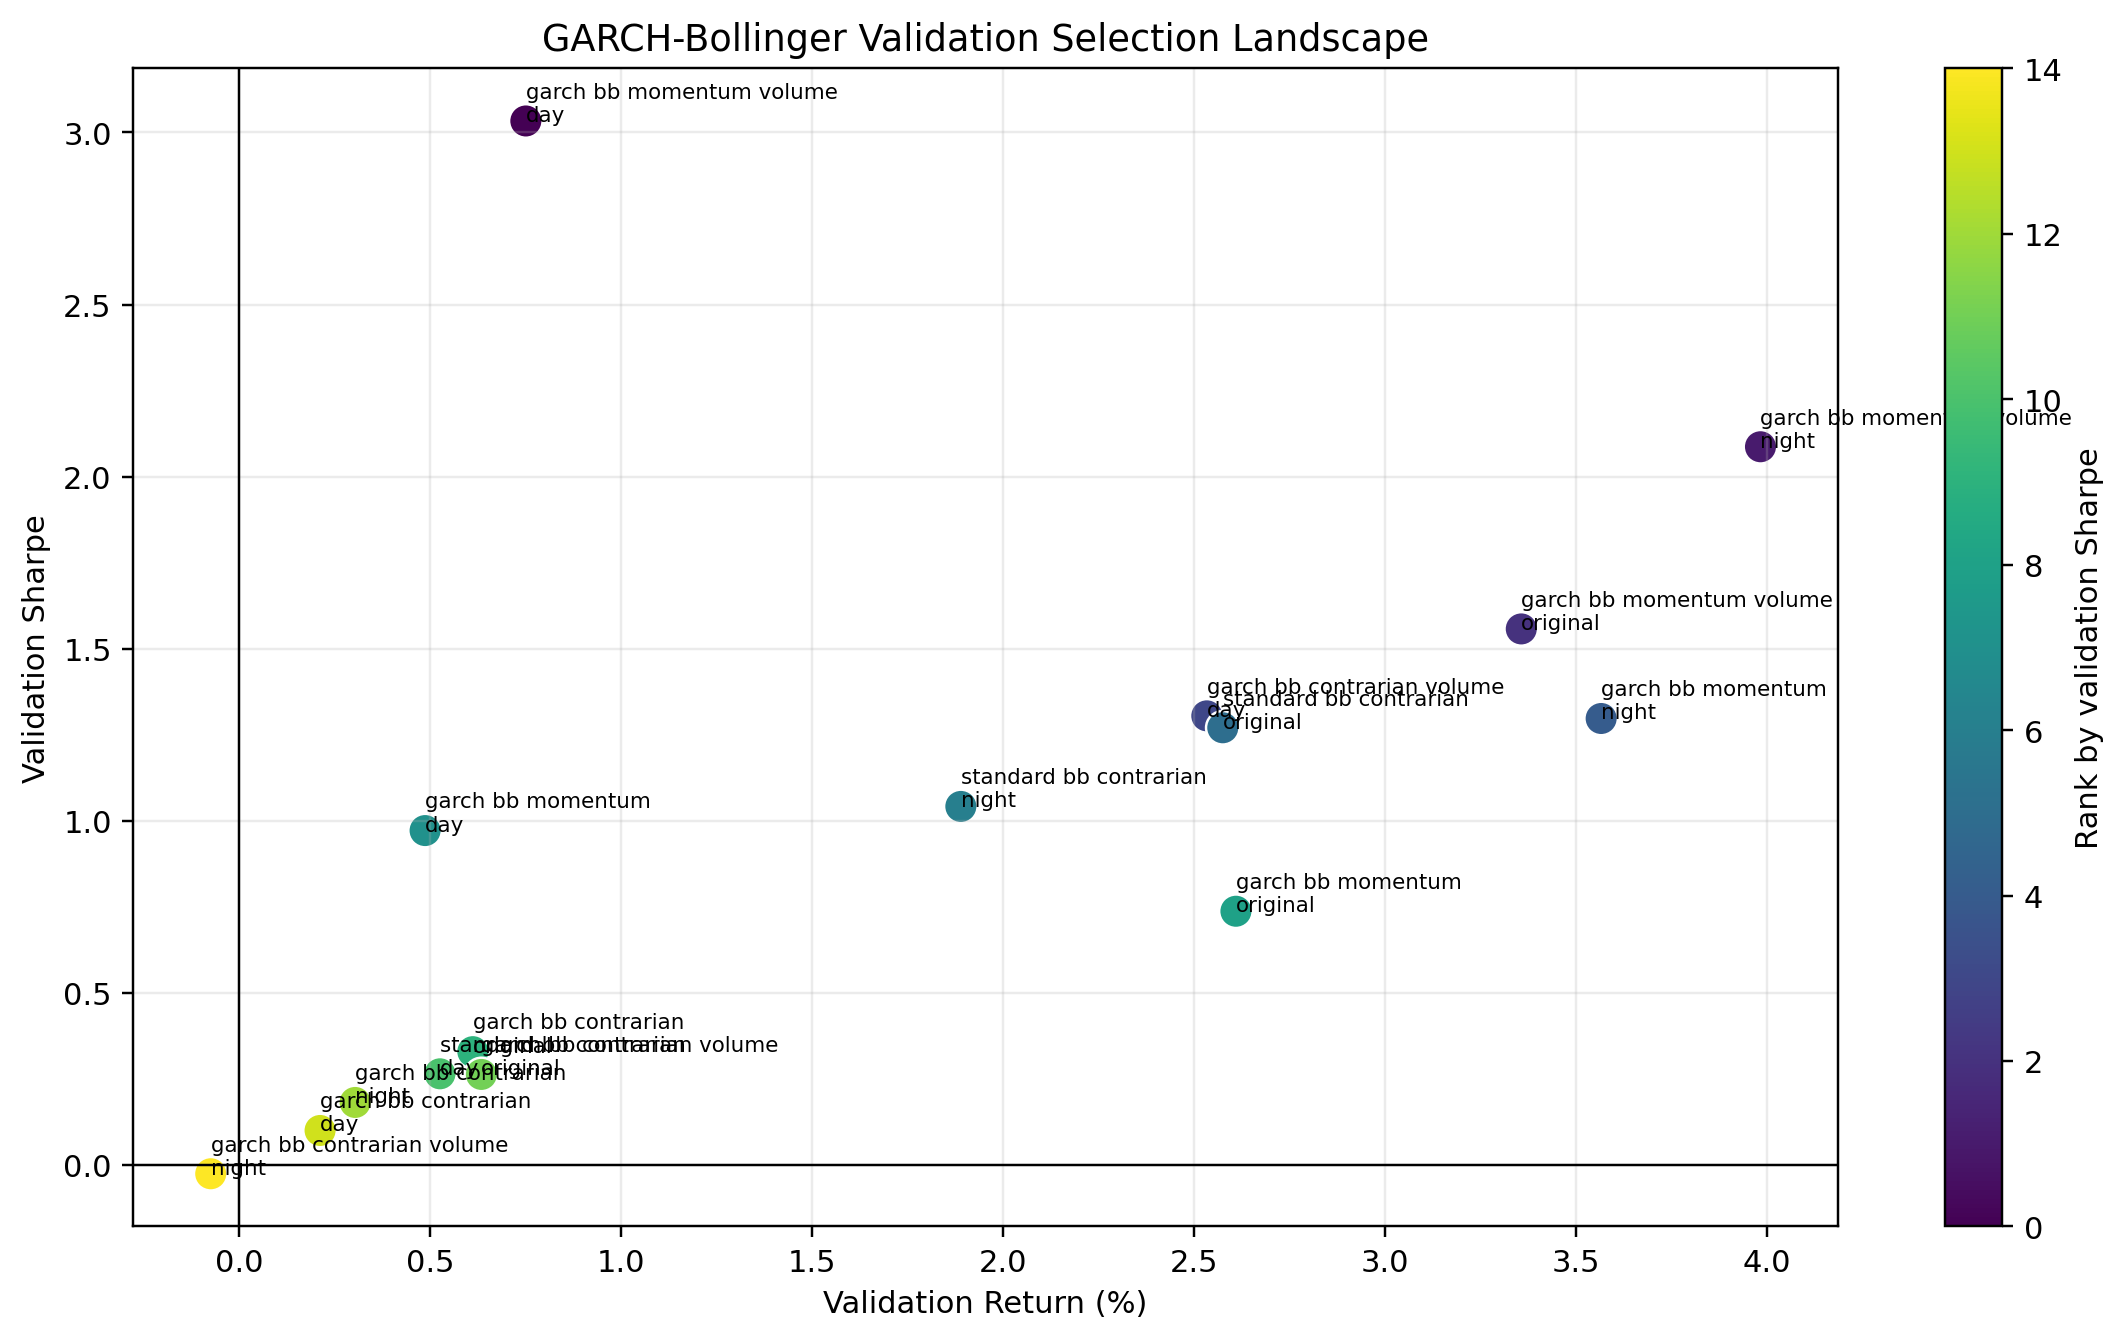
\includegraphics[width=0.9\textwidth]{garch_validation_selection.png}
    \caption{Validation selection landscape for GARCH-Bollinger candidates. The plot illustrates that validation performance is highly parameter- and regime-dependent.}
    \label{fig:garch-validation}
\end{figure}

The key methodological point is that test performance does not feed back into parameter selection. This protects the final test period from data snooping.

\section{Backtesting, Slippage and Risk Management}

\subsection{Backtesting Assumptions}

The backtests include transaction cost and slippage proxies. The common futures assumptions are:

\begin{table}[H]
    \centering
    \caption{Main trading assumptions.}
    \label{tab:trading-assumptions}
    \begin{tabular}{lr}
        \toprule
        Item & Value \\
        \midrule
        Initial capital & HKD 5,000,000 \\
        HSI futures multiplier & HKD 50 per index point \\
        Slippage proxy & 1 index point \\
        GRPO transaction cost & HKD 10 per contract \\
        LGBM transaction cost rate & 0.01\% per side \\
        \bottomrule
    \end{tabular}
\end{table}

The accounting conventions differ across implementations. GRPO reports HKD PnL using futures multiplier and initial capital. LGBM reports return-based metrics and also has a separate risk-management module. GARCH-Bollinger reports ratio returns for the technical strategy tests. Therefore, the results should be compared directionally rather than treated as perfectly identical measurement systems.

\subsection{LGBM Backtesting Results}

The LGBM test results are strong across most scenarios, especially for the original model tested on original, day and night datasets.

\begin{figure}[H]
    \centering
    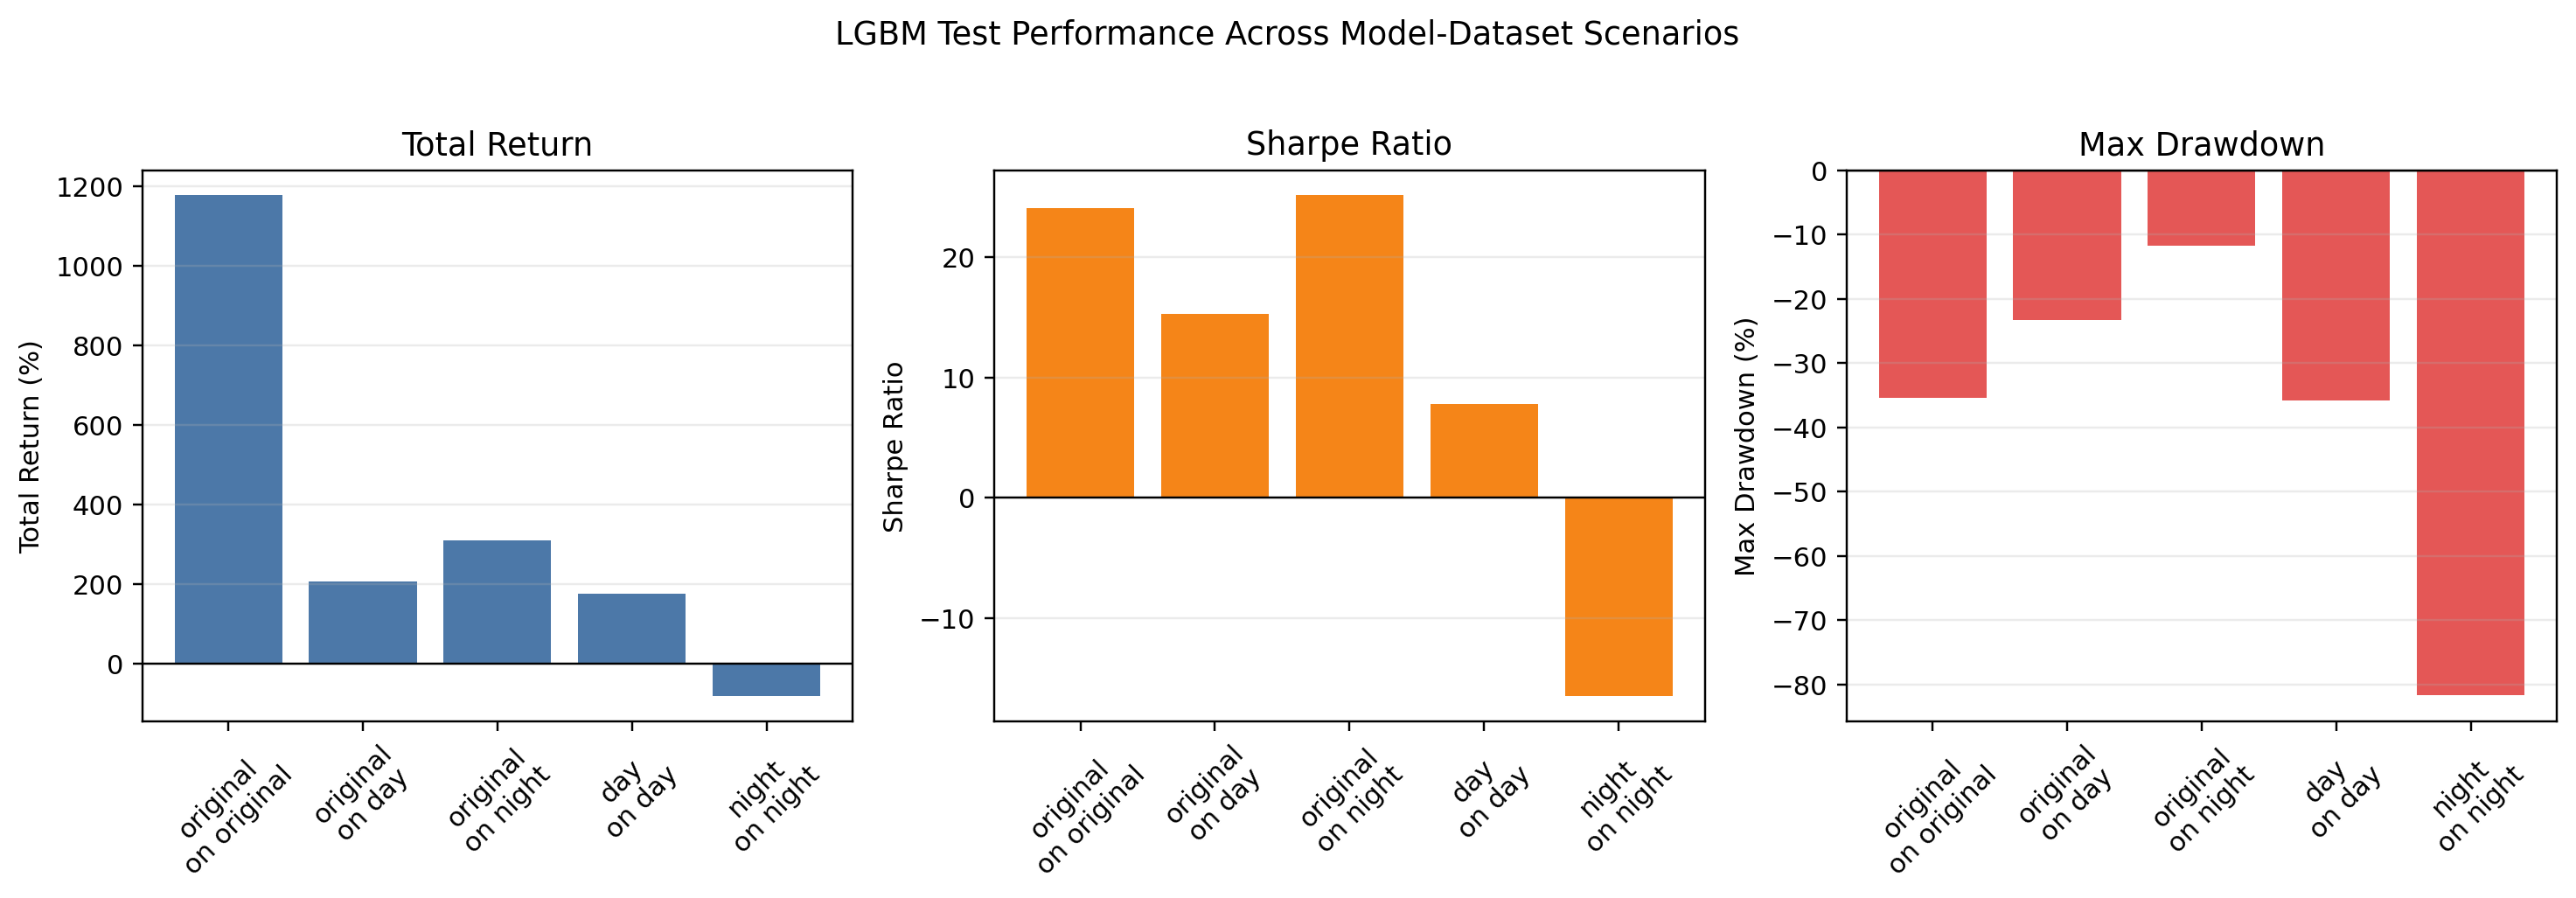
\includegraphics[width=0.98\textwidth]{lgbm_test_performance.png}
    \caption{LGBM test performance by scenario. The original model generalizes better than the night-specific model in this experiment.}
    \label{fig:lgbm-performance}
\end{figure}

\begin{table}[H]
    \centering
    \caption{LGBM test metrics.}
    \label{tab:lgbm-test}
    \begin{tabular}{lrrrr}
        \toprule
        Scenario & Total Return & Sharpe & Max DD & Trades \\
        \midrule
        Original on original & 1177.73\% & 24.07 & -35.44\% & 6584 \\
        Original on day & 207.85\% & 15.29 & -23.35\% & 4016 \\
        Original on night & 311.09\% & 25.13 & -11.80\% & 2599 \\
        Day on day & 176.40\% & 7.78 & -35.81\% & 4964 \\
        Night on night & -81.63\% & -16.51 & -81.67\% & 7032 \\
        \bottomrule
    \end{tabular}
\end{table}

The poor performance of the night-specific model suggests overfitting, regime instability, or insufficient robustness in night-session signals. The LGBM risk-management module is more conservative than the raw backtest. It reports final capital of HKD 8.57 million, total return of 71.44\%, maximum drawdown of -4.30\%, 2704 trades, and win rate of 66.72\%.

\subsection{GRPO Backtesting Results}

The fixed one-contract GRPO evaluation is weak before adding dynamic risk management. The least negative fixed case is \texttt{day\_model} on \texttt{day\_test}, but it still loses HKD 154,570 with Sharpe ratio -0.83.

\begin{figure}[H]
    \centering
    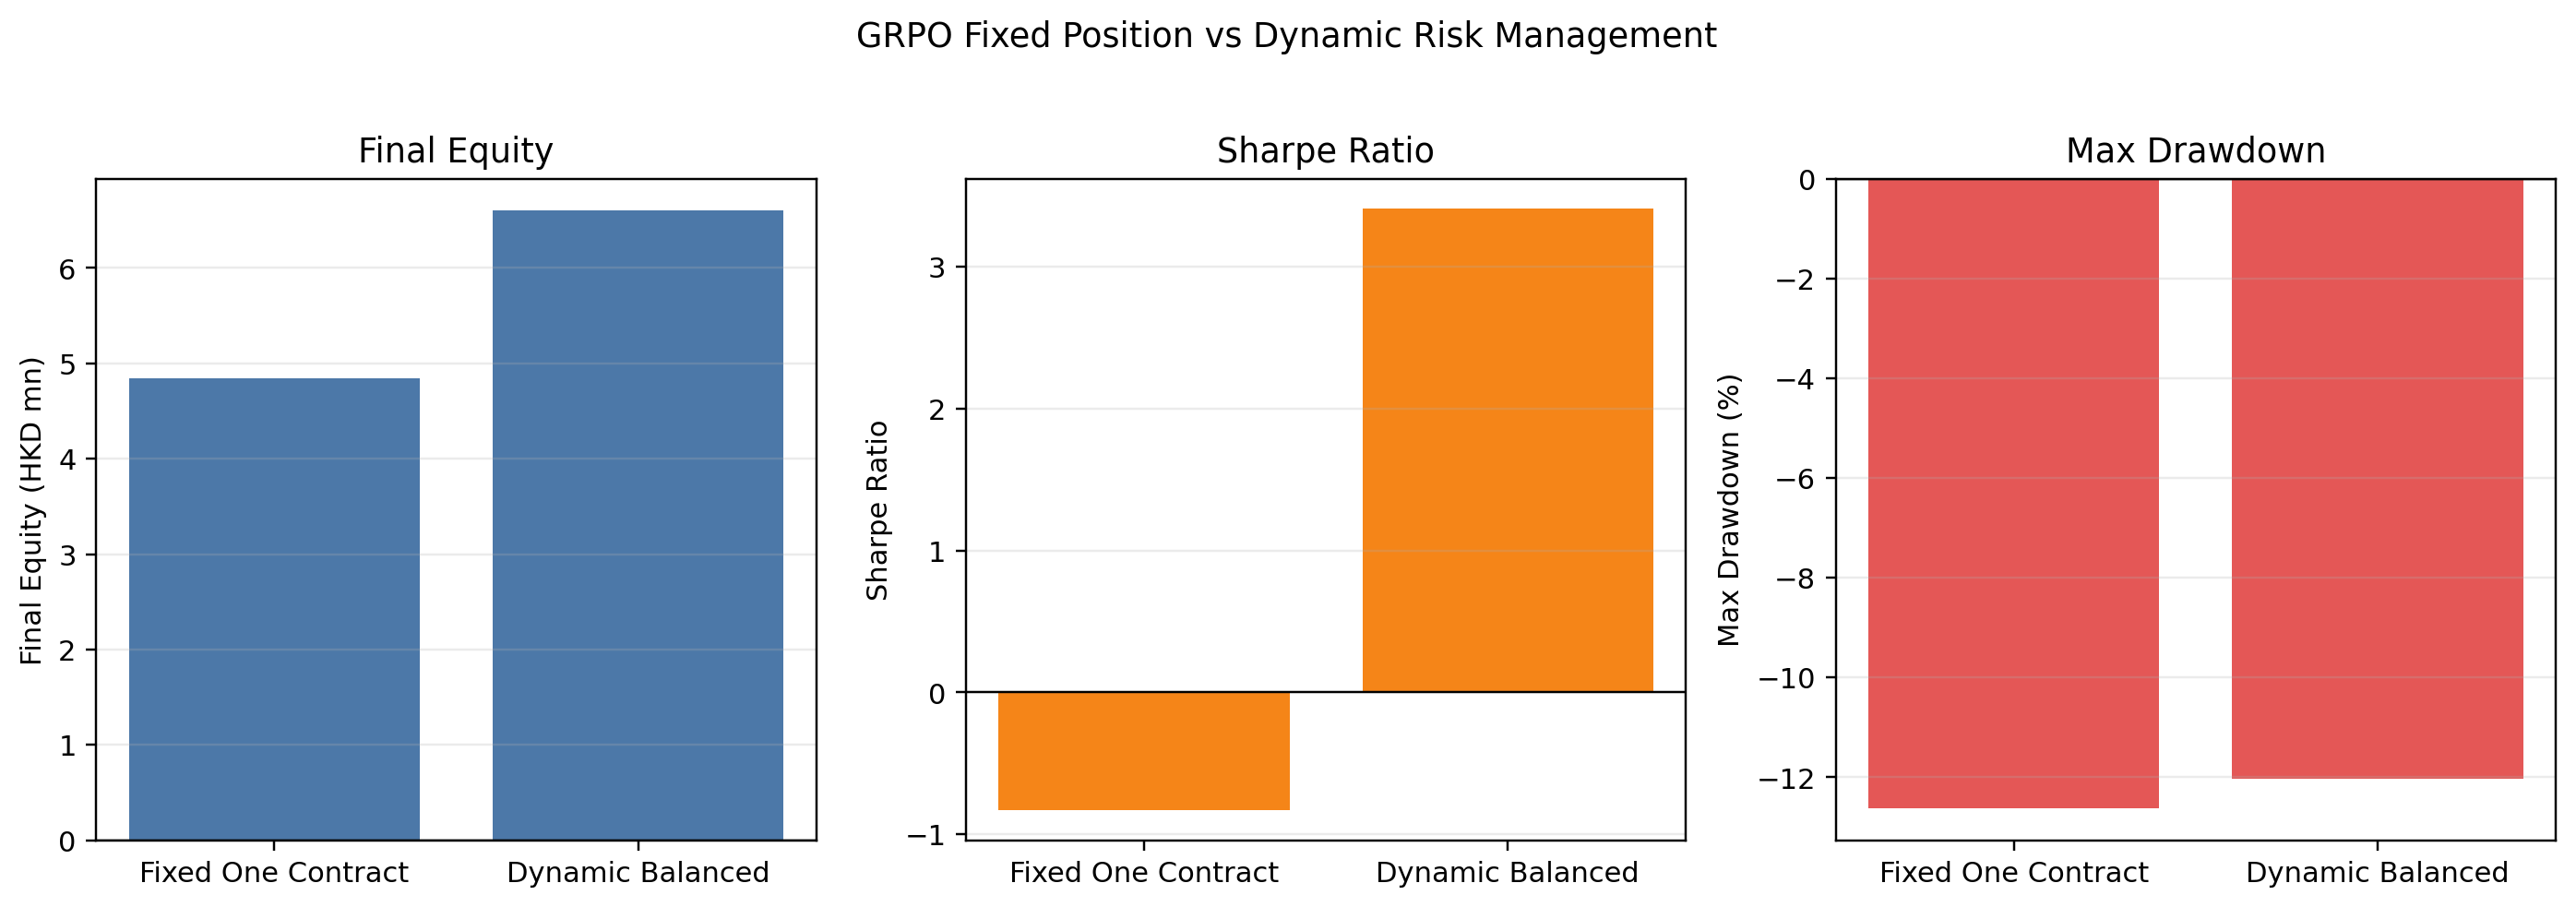
\includegraphics[width=0.94\textwidth]{grpo_risk_comparison.png}
    \caption{GRPO fixed one-contract baseline versus dynamic balanced risk management. Dynamic position sizing changes both return and risk characteristics.}
    \label{fig:grpo-risk}
\end{figure}

\begin{table}[H]
    \centering
    \caption{GRPO risk comparison.}
    \label{tab:grpo-risk}
    \begin{tabular}{lrrrrr}
        \toprule
        Method & Final Equity & Total PnL & Sharpe & Max DD & Trades \\
        \midrule
        Fixed one contract & 4,845,430 & -154,570 & -0.83 & -12.63\% & 7704 \\
        Dynamic balanced & 6,607,190 & 1,607,190 & 3.41 & -12.04\% & 4188 \\
        \bottomrule
    \end{tabular}
\end{table}

The dynamic layer sizes positions using equity risk budget and recent volatility, reduces maximum contracts in protective drawdown mode, stops new trades under a kill switch, applies stop-loss and take-profit rules, and uses cooldown bars after stop-loss events.

\begin{figure}[H]
    \centering
    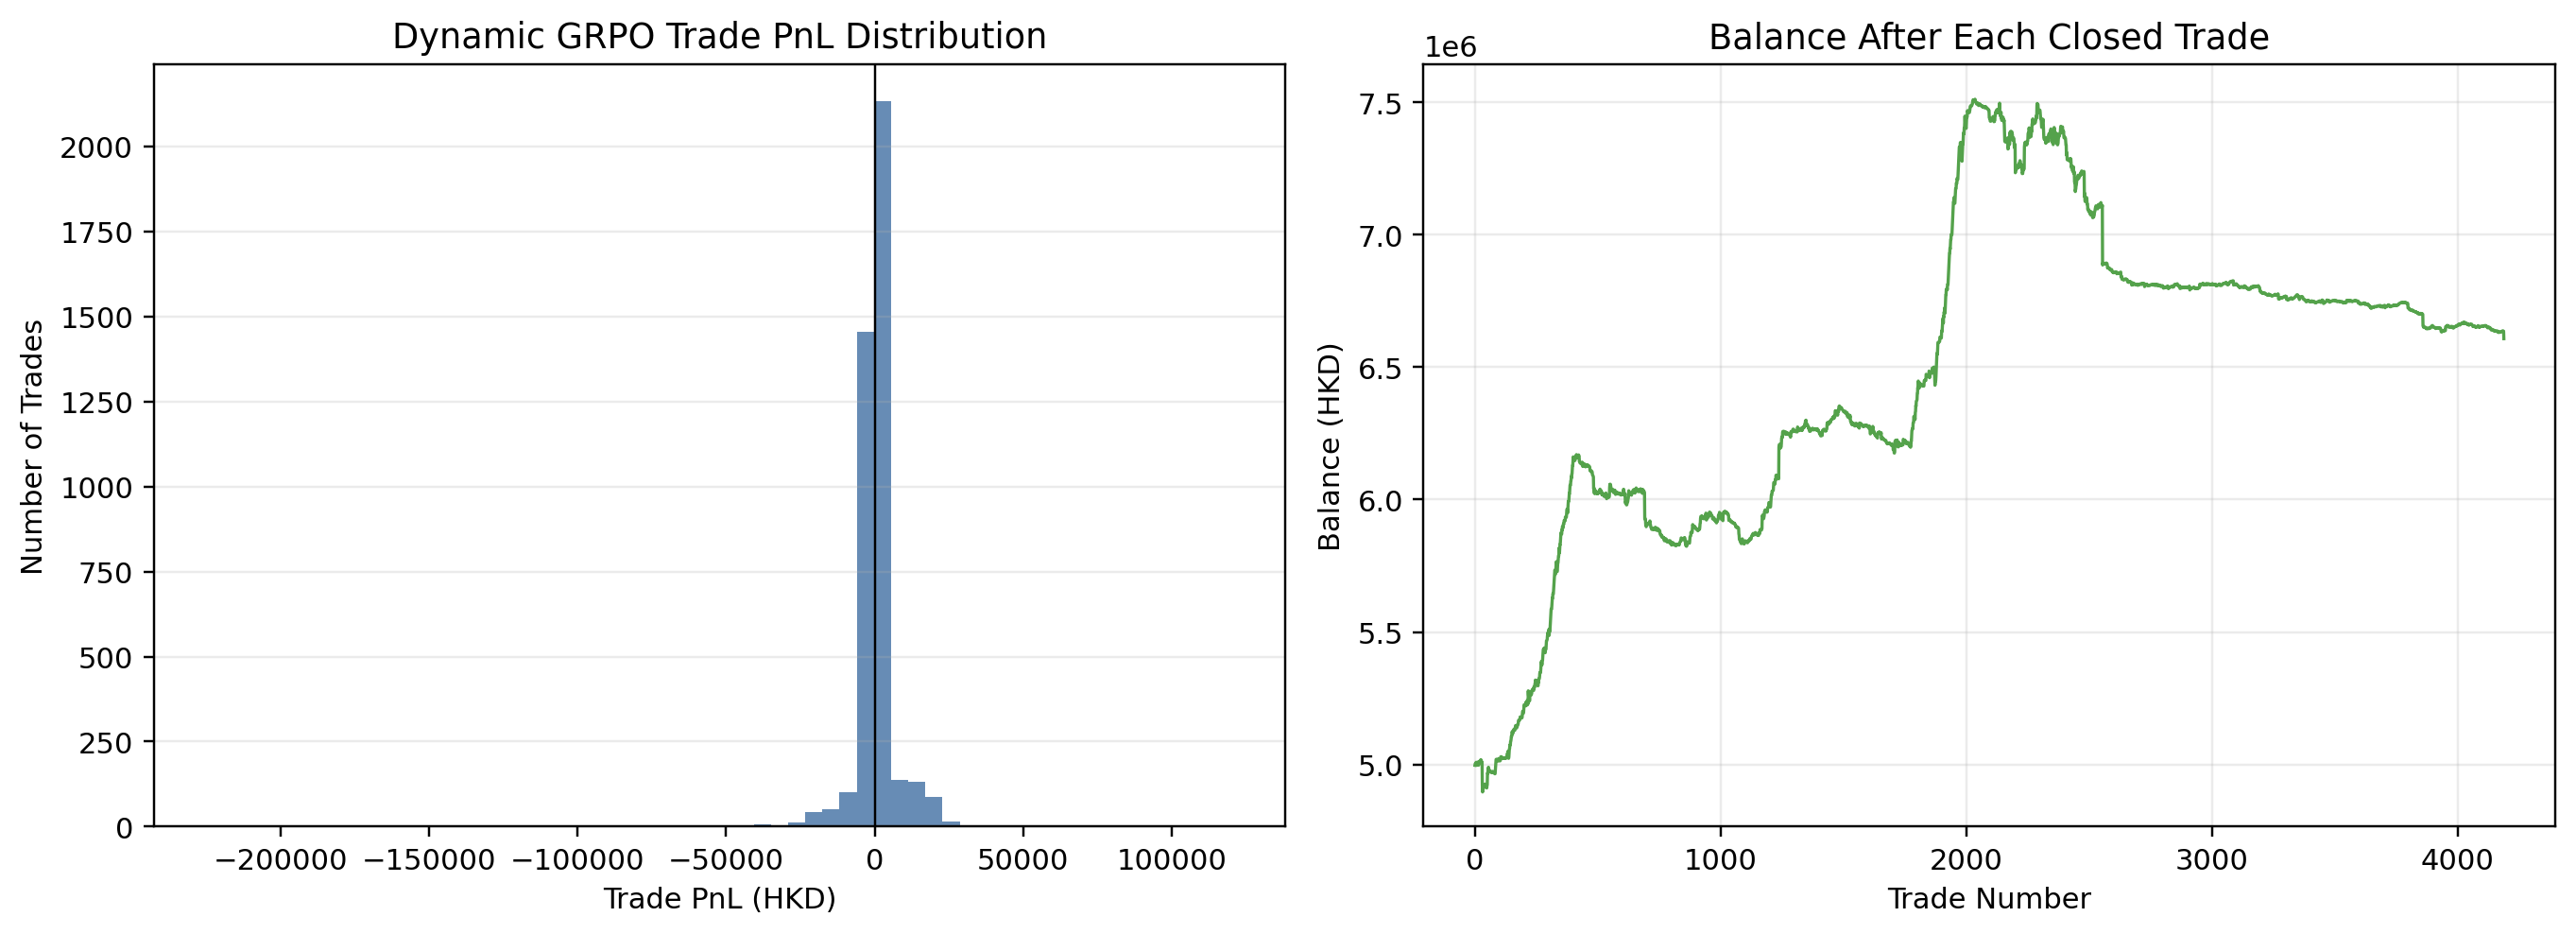
\includegraphics[width=0.95\textwidth]{dynamic_trade_pnl.png}
    \caption{Dynamic GRPO trade PnL distribution and balance after each closed trade. The distribution shows frequent small trades with occasional large stop-loss events.}
    \label{fig:dynamic-trades}
\end{figure}

\subsection{GARCH-Bollinger Backtesting Results}

The GARCH-Bollinger validation results favored momentum strategies with volume confirmation, but out-of-sample test results were more favorable to contrarian rules. This is an important regime-risk result.

\begin{figure}[H]
    \centering
    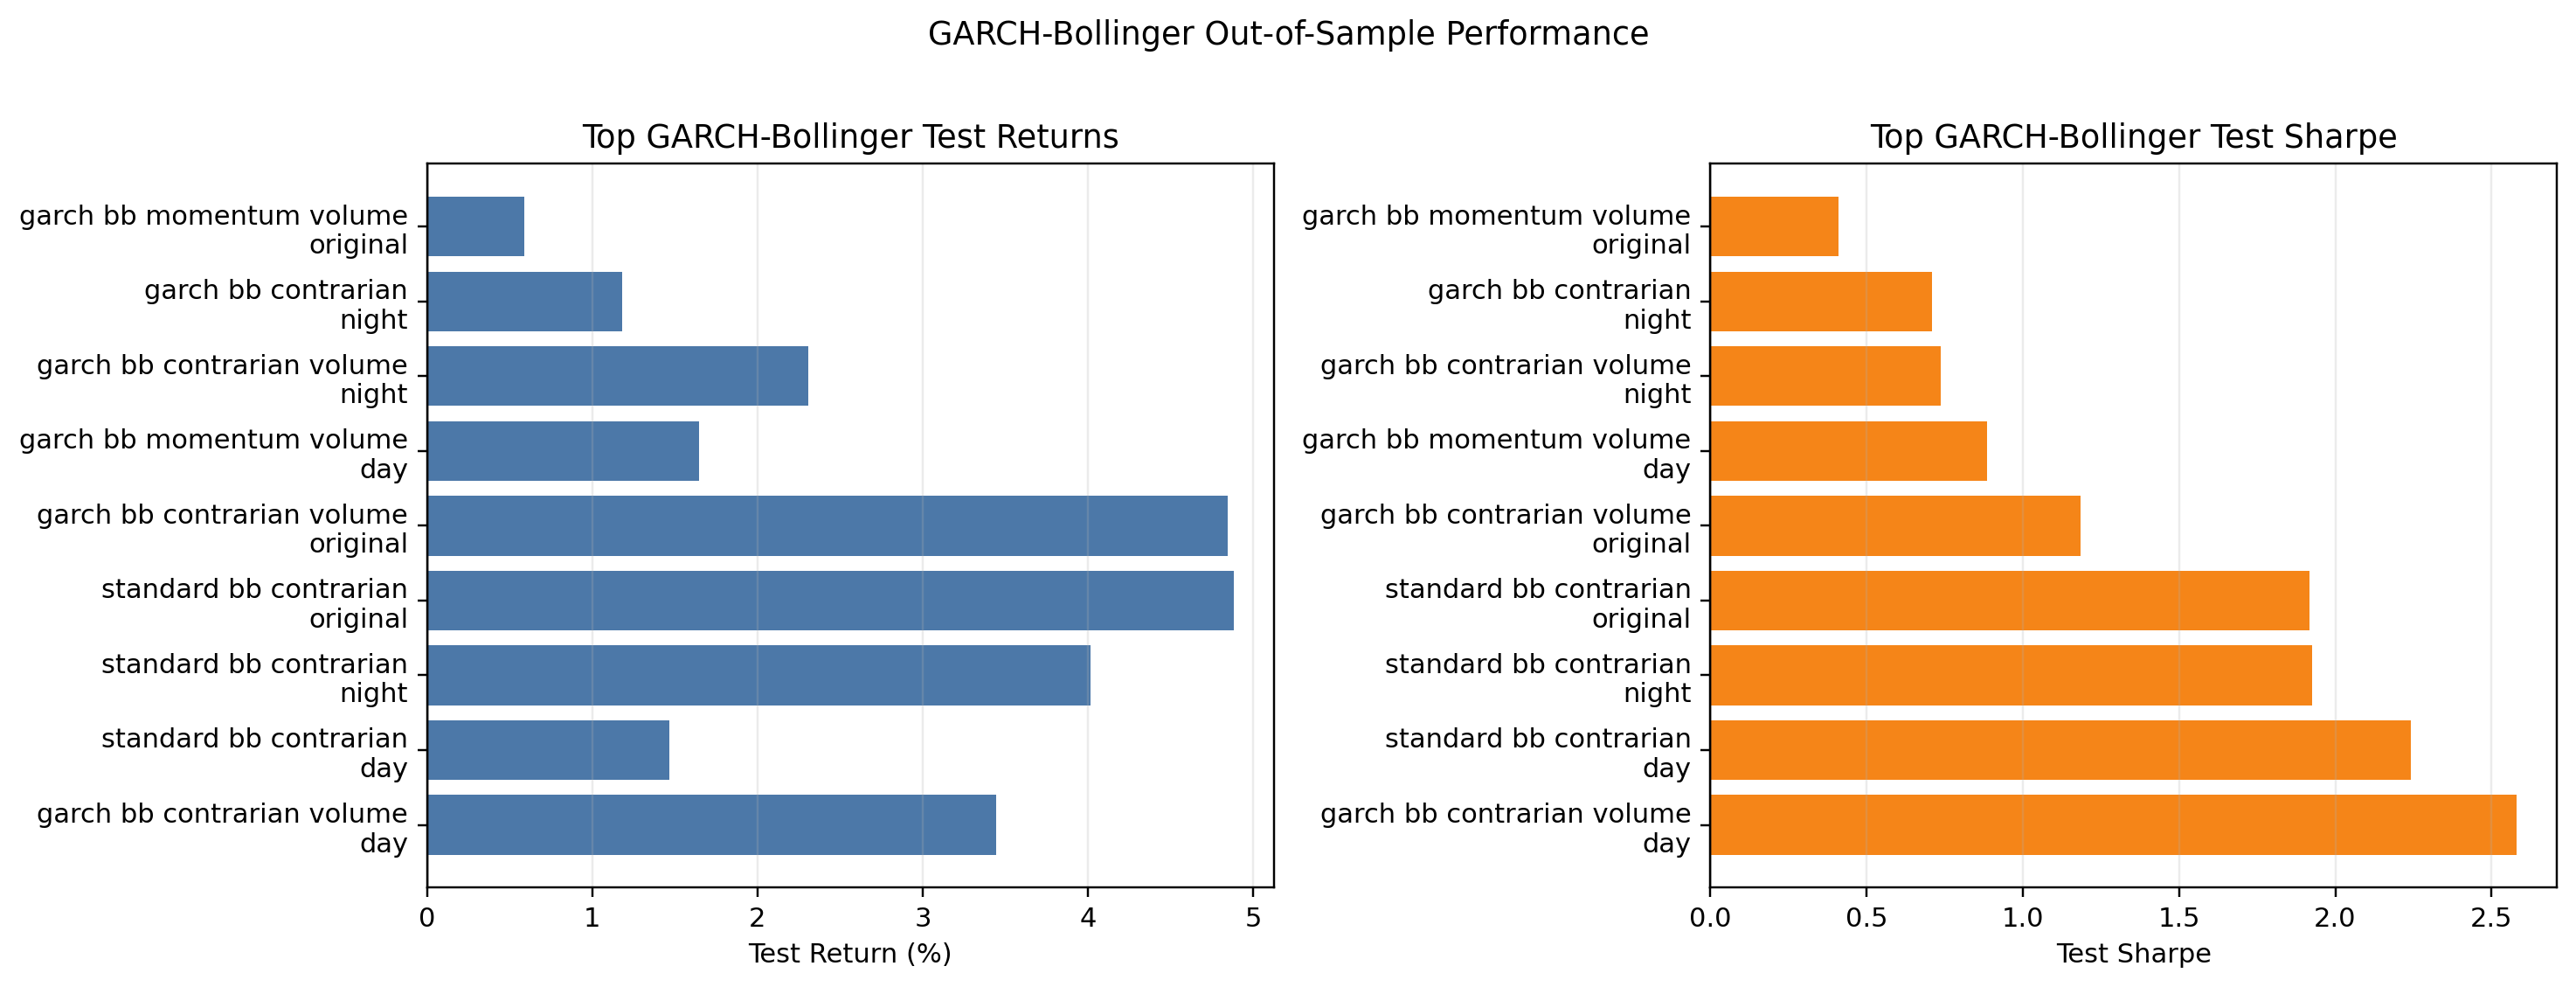
\includegraphics[width=0.98\textwidth]{garch_test_results.png}
    \caption{Top GARCH-Bollinger out-of-sample results. Contrarian variants dominate many of the strongest test cases.}
    \label{fig:garch-test}
\end{figure}

\begin{table}[H]
    \centering
    \caption{Representative GARCH-Bollinger test results.}
    \label{tab:garch-test}
    \begin{tabular}{llrrr}
        \toprule
        Variant & Test Dataset & Return & Sharpe & Max DD \\
        \midrule
        Standard BB contrarian & Original & 4.88\% & 1.92 & -2.13\% \\
        Standard BB contrarian & Day & 1.47\% & 2.24 & -0.58\% \\
        Standard BB contrarian & Night & 4.02\% & 1.93 & -2.13\% \\
        GARCH BB contrarian volume & Day & 3.44\% & 1.96 & -1.43\% \\
        GARCH BB momentum volume & Day & 1.64\% & 0.89 & -1.97\% \\
        \bottomrule
    \end{tabular}
\end{table}

The result is not simply that GARCH is always better than standard Bollinger Bands, or that momentum is always worse than contrarian trading. A more precise interpretation is that the validation period behaved more like a breakout environment, while the test period, especially late 2019 to early 2020, was more favorable to mean reversion after band breaches.

\subsection{Slippage Discussion}

The project models slippage with a simplified one-point proxy. In live trading, slippage depends on order type, queue position, bid-ask spread, market depth, volatility, news timing, and whether the strategy needs to reverse directly from long to short or short to long. Slippage can be larger during night sessions, market open and close, lunch break restart, macro news, overseas shocks, and large price gaps. Therefore, the backtest should be interpreted as a bar-level execution approximation, not a full order-book simulation.

\subsection{Risk Management Features}

The project implements risk management at several levels. For LGBM, the risk manager controls position sizing, maximum exposure, single-trade loss, daily drawdown, and consecutive-loss halt. For GRPO, the dynamic module uses risk budget, maximum contracts, protective drawdown, kill switch, stop-loss, take-profit, cooldown bars, volatility lookback, and minimum volatility assumptions. For GARCH-Bollinger, risk control is simpler but still present through band width, volume confirmation, maximum holding bars, and transaction-cost-adjusted returns.

\begin{table}[H]
    \centering
    \caption{Main dynamic risk parameters for GRPO.}
    \label{tab:risk-params}
    \begin{tabular}{lr}
        \toprule
        Parameter & Value \\
        \midrule
        Risk per trade & 0.5\% of equity \\
        Maximum contracts & 5 \\
        Protective drawdown & 8\% \\
        Kill-switch drawdown & 12\% \\
        Stop-loss multiple & 1.0 risk budget \\
        Take-profit multiple & 1.5 risk budget \\
        Cooldown bars & 20 \\
        Volatility lookback & 60 bars \\
        Minimum volatility points & 20 \\
        \bottomrule
    \end{tabular}
\end{table}

\section{Real-Time Implementation Difficulties}

The current project is a research and backtesting framework, not a production trading system. A live implementation would face several practical problems.

First, real-time data quality is harder than historical CSV backtesting. A live system must detect missing bars, delayed ticks, duplicated bars, lunch breaks, night-session boundaries, holidays, and abnormal timestamps. If live session handling differs from the backtest, rolling indicators, GARCH volatility, LGBM features, and GRPO observations may become inconsistent.

Second, signals should be generated only from completed bars. Using unfinished one-minute bars creates hidden look-ahead bias because high, low, close, and volume are not final yet.

Third, futures trading has contract lifecycle issues. HSI futures have expiry months, rollover dates, and liquidity migration from the expiring contract to the next active contract. A production system must decide when to roll and how to handle price gaps between contracts.

Fourth, margin and forced liquidation are central to futures trading. A broker imposes initial margin, maintenance margin, intraday checks, and liquidation rules. A sharp adverse move can trigger margin calls before the model's intended stop-loss logic is reached.

Finally, a live system needs operational controls: kill switch, daily loss limit, order throttling, broker-position reconciliation, logging, alerting, and manual override.

\section{Additional Discussion}

The three strategies have different strengths and weaknesses. LGBM produces the strongest raw test performance, but the extremely high returns and Sharpe ratios should be interpreted carefully because intraday machine learning backtests are vulnerable to overfitting, subtle leakage, and optimistic execution assumptions. GRPO is conceptually attractive because it optimizes trading actions directly, but the raw fixed-contract policy is not profitable in this experiment. Its value appears only after dynamic position sizing and risk controls are added. GARCH-Bollinger is the most interpretable strategy. Its returns are less spectacular, but it clearly illustrates regime risk: validation favored momentum, while the final test period favored contrarian rules.

Overall, the project supports a cautious view of quantitative strategy development. A strong backtest is not enough. A credible trading strategy must also have a clear economic rationale, clean data splitting, realistic cost assumptions, robust out-of-sample testing, and risk management that can survive adverse market regimes.

\section{Conclusion}

This project compares supervised learning, reinforcement learning, and traditional volatility-based technical trading on intraday HSI futures data. The LGBM strategy achieves the strongest raw test performance, especially for the original model, but its results require careful interpretation because high-frequency prediction is sensitive to overfitting and execution assumptions. The GRPO strategy performs poorly under fixed one-contract trading, but the dynamic balanced risk-management layer significantly improves its final equity and Sharpe ratio. The GARCH-Bollinger strategy is more interpretable and shows that contrarian band-breach rules can be more robust than validation-selected momentum rules in the final test period.

The main lesson is that model complexity alone does not guarantee trading robustness. The final strategy quality depends on the full pipeline: data cleaning, chronological splitting, feature construction, validation discipline, transaction cost modeling, position sizing, drawdown control, and implementation feasibility. For real deployment, the next steps should include more conservative execution simulation, walk-forward validation, live paper trading, and broker-level risk-control integration.

\section*{References}
\addcontentsline{toc}{section}{References}

\begin{enumerate}
    \item Bollinger, J. (2002). \textit{Bollinger on Bollinger Bands}. McGraw-Hill.
    \item Engle, R. F. (1982). Autoregressive conditional heteroscedasticity with estimates of the variance of United Kingdom inflation. \textit{Econometrica}, 50(4), 987-1007.
    \item Fama, E. F. (1970). Efficient capital markets: A review of theory and empirical work. \textit{Journal of Finance}, 25(2), 383-417.
    \item Ke, G., Meng, Q., Finley, T., Wang, T., Chen, W., Ma, W., Ye, Q., and Liu, T. Y. (2017). LightGBM: A highly efficient gradient boosting decision tree. \textit{Advances in Neural Information Processing Systems}.
    \item Sutton, R. S., McAllester, D., Singh, S., and Mansour, Y. (1999). Policy gradient methods for reinforcement learning with function approximation. \textit{Advances in Neural Information Processing Systems}.
    \item Hong Kong Exchanges and Clearing Limited (HKEX). Hang Seng Index Futures contract specifications and trading information.
\end{enumerate}

\end{document}
